\section{Results and Discussion}
\label{sec:results}
We report two configurations that use the identical split, prompt, parser and metrics. \textbf{Configuration~A} (GPU, Kaggle T4) fine-tunes SmolLM2-1.7B as target with SmolLM2-360M as draft and carries the headline accuracy results; \textbf{Configuration~B} (CPU, laptop) uses the 360M target with the 135M draft and is the model that the locally hosted application loads by default (Section~\ref{sec:cpu}). All numbers below come from files written by the scripts in the repository.

\subsection{Fine-Tuning and Model Selection (Config.~A)}
Table~\ref{tab:epochsA} lists validation behaviour after each epoch and Fig.~\ref{fig:trainA} the training curves. Answer-token training loss falls from about 0.40 to about 0.12 for the 1.7B target, and validation loss falls from 0.190 to 0.155 between epochs 1 and 2 and then stays flat (0.156). Validation macro-F1 peaks at epoch \GTBestEpoch{} (0.365) and drops at epoch 3 (0.326), and validation accuracy follows the same pattern (0.714 vs.\ 0.694), so the epoch-2 adapter was kept for the target; the same criterion selected epoch \GDBestEpoch{} for the 360M draft (Table~\ref{tab:epochsAd}). Because macro-F1 over six classes on 206 validation rows is noisy (the curves in Fig.~\ref{fig:trainA} move by several points between epochs while the loss is flat), the selection is made on a weak signal; we report it as observed rather than as a tuned optimum. Training took \GTTrainHours{}\,h (target) and \GDTrainHours{}\,h (draft) on one T4 with fp16 autocast, micro-batch 1 and 16 accumulation steps for the 1.7B model (to fit 15\,GB), and micro-batch 4 with 4 accumulation steps for the draft; the effective batch is 16 in both cases.

\begin{table}[t]\centering\caption{Config.~A target (SmolLM2-1.7B + LoRA): validation after each epoch ($^*$ = selected).}\label{tab:epochsA}
\small\begin{tabular}{rrrrr}\toprule
Epoch & Val. loss & Val. acc. & Val. macro-F1 & Val. evid. F1 \\\midrule
1 & 0.190 & 0.675 & 0.309 & 0.306 \\
2$^*$ & 0.155 & 0.714 & 0.365 & 0.374 \\
3 & 0.156 & 0.694 & 0.326 & 0.391 \\
\bottomrule\end{tabular}
\end{table}
\begin{table}[t]\centering\caption{Config.~A draft (SmolLM2-360M + LoRA): validation after each epoch.}\label{tab:epochsAd}
\small\begin{tabular}{rrrrr}\toprule
Epoch & Val. loss & Val. acc. & Val. macro-F1 & Val. evid. F1 \\\midrule
1 & 0.220 & 0.621 & 0.215 & 0.124 \\
2$^*$ & 0.192 & 0.718 & 0.341 & 0.325 \\
3 & 0.186 & 0.641 & 0.259 & 0.063 \\
4 & 0.184 & 0.689 & 0.323 & 0.262 \\
\bottomrule\end{tabular}
\end{table}
\begin{figure}[t]\centering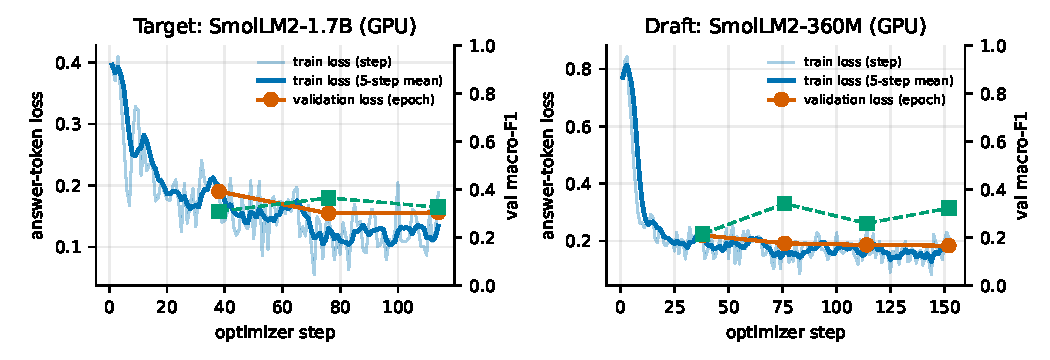
\includegraphics[width=\columnwidth]{gpu_fig_training.pdf}
\caption{Config.~A training curves: step and smoothed training loss, epoch-level validation loss (red) and validation macro-F1 (green, right axis).}\label{fig:trainA}\end{figure}

\subsection{Before and After Fine-Tuning (Config.~A)}
Table~\ref{tab:mainA} compares, on \emph{identical} validation and test rows with the same prompt, greedy decoding and parser, a trivial majority-label baseline, the base model used zero-shot, and the fine-tuned model; Fig.~\ref{fig:baA} visualises the test columns. The base model is almost never right: test accuracy \GBaseAcc{} (95\% patient-bootstrap interval \GBaseAccLo--\GBaseAccHi) and macro-F1 \GBaseMF{}. Its outputs are well-formed JSON (only \GBaseInvalid{} invalid output), so the failure is semantic: it commits to a decisive label, and on all 131 exclusion rows it never produces the correct one (exclusion accuracy 0.000). Fine-tuning lifts test accuracy to \GTestAcc{} (interval \GTestAccLo--\GTestAccHi) and macro-F1 to \GTestMF{} (interval \GTestMFLo--\GTestMFHi), with no invalid outputs.

Two cautions are needed to read this correctly. First, a trivial predictor already attains \GMajAcc{} accuracy on the test split because \emph{not excluded} and \emph{not enough information} dominate; the accuracy interval of the fine-tuned model (lower end \GTestAccLo) therefore overlaps the majority baseline, so we cannot claim a statistically supported accuracy gain over guessing the common label. The macro-F1 gain is clearer (0.460 vs.\ 0.272, interval lower end \GTestMFLo), because macro-F1 rewards the minority classes. Second, the gain is entirely on inclusion criteria: inclusion accuracy rises from the majority baseline's 0.507 to 0.747 and macro-F1 from 0.168 to 0.516, whereas exclusion accuracy (0.687) is \emph{below} the majority baseline's 0.695 and macro-F1 is unchanged (0.271 vs.\ 0.273). The reason is visible in the confusion matrices below: for exclusion criteria the model predicts \emph{not excluded} for 130 of 131 rows.

\begin{table*}[t]\centering\caption{Config.~A: majority baseline, base zero-shot and fine-tuned SmolLM2-1.7B on the same rows (acc.\ = accuracy, mF1 = macro-F1; Invalid = unparseable outputs).}\label{tab:mainA}
\small\begin{tabular}{llrrrrrrr}\toprule
Split & Model & Acc. & mF1 & Incl. acc. & Incl. mF1 & Excl. acc. & Excl. mF1 & Invalid \\\midrule
Val. & majority label & 0.621 & 0.215 & 0.409 & 0.145 & 0.721 & 0.210 & 0 \\
& base zero-shot & 0.170 & 0.131 & 0.500 & 0.206 & 0.014 & 0.007 & 0 \\
& fine-tuned & 0.714 & 0.365 & 0.667 & 0.344 & 0.736 & 0.269 & 0 \\
\midrule
Test & majority label & 0.626 & 0.272 & 0.507 & 0.168 & 0.695 & 0.273 & 0 \\
& base zero-shot & 0.146 & 0.111 & 0.400 & 0.182 & 0.000 & 0.000 & 1 \\
& fine-tuned & 0.709 & 0.460 & 0.747 & 0.516 & 0.687 & 0.271 & 0 \\
\bottomrule\end{tabular}
\end{table*}
\begin{figure}[t]\centering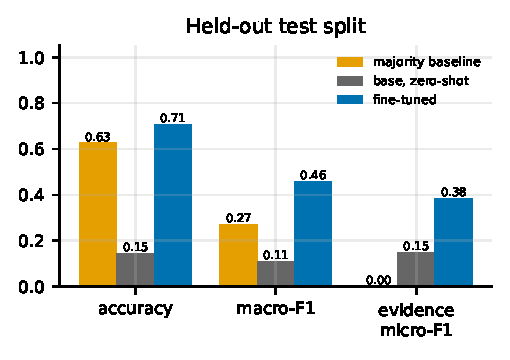
\includegraphics[width=.8\columnwidth]{gpu_fig_before_after.pdf}
\caption{Config.~A test results: majority baseline, base zero-shot and fine-tuned model.}\label{fig:baA}\end{figure}

\subsection{Per-Class Results and Inclusion vs.\ Exclusion (Config.~A)}
Table~\ref{tab:pcA} and Fig.~\ref{fig:cmA} give per-class precision, recall and F1 and the confusion matrices overall and by criterion type (rows are expert labels, columns predictions). \emph{Included} is handled well (P 0.79, R 0.70, F1 0.75 on 27 rows) and \emph{not excluded} has high recall (0.99) but only 0.69 precision because 28 \emph{not enough information} and 12 \emph{not applicable} exclusion rows are also labelled \emph{not excluded}. \emph{Not enough information} reaches F1 0.62 (inclusion: 36 of 38 correct), \emph{not applicable} has precision 1.0 but recall 0.07 (1 of 15), and \emph{not included} (7 rows) is never predicted. The \emph{excluded} class has no test support, so it contributes neither to recall nor to macro-F1 (Section~IV-B). The base model's per-class table (Table~\ref{tab:pcB}) shows the contrast: it spreads predictions over decisive labels with near-zero precision. Table~\ref{tab:pcA} should therefore be read as: reliable on \emph{included} and \emph{not enough information} for inclusion criteria, essentially majority-class behaviour for exclusion criteria, and no ability on the rarest classes.

\begin{table}[t]\centering\caption{Config.~A fine-tuned model, test split: per-class precision (P), recall (R), F1 and support.}\label{tab:pcA}
\footnotesize\begin{tabular}{llrrrr}\toprule
Scope & Class & P & R & F1 & Support \\\midrule
inclusion & included & 0.792 & 0.704 & 0.745 & 27 \\
 & not included & 0.000 & 0.000 & 0.000 & 7 \\
 & not enough info. & 0.720 & 0.947 & 0.818 & 38 \\
 & not applicable & 1.000 & 0.333 & 0.500 & 3 \\
\midrule
exclusion & excluded & 0.000 & 0.000 & 0.000 & 0 \\
 & not excluded & 0.692 & 0.989 & 0.814 & 91 \\
 & not enough info. & 0.000 & 0.000 & 0.000 & 28 \\
 & not applicable & 0.000 & 0.000 & 0.000 & 12 \\
\bottomrule\end{tabular}
\end{table}
\begin{table}[t]\centering\caption{Config.~A base model (zero-shot), test split.}\label{tab:pcB}
\footnotesize\begin{tabular}{llrrrr}\toprule
Scope & Class & P & R & F1 & Support \\\midrule
inclusion & included & 0.409 & 1.000 & 0.581 & 27 \\
 & not included & 0.000 & 0.000 & 0.000 & 7 \\
 & not enough info. & 1.000 & 0.079 & 0.146 & 38 \\
 & not applicable & 0.000 & 0.000 & 0.000 & 3 \\
\midrule
exclusion & excluded & 0.000 & 0.000 & 0.000 & 0 \\
 & not excluded & 0.000 & 0.000 & 0.000 & 91 \\
 & not enough info. & 0.000 & 0.000 & 0.000 & 28 \\
 & not applicable & 0.000 & 0.000 & 0.000 & 12 \\
\bottomrule\end{tabular}
\end{table}
\begin{figure*}[t]\centering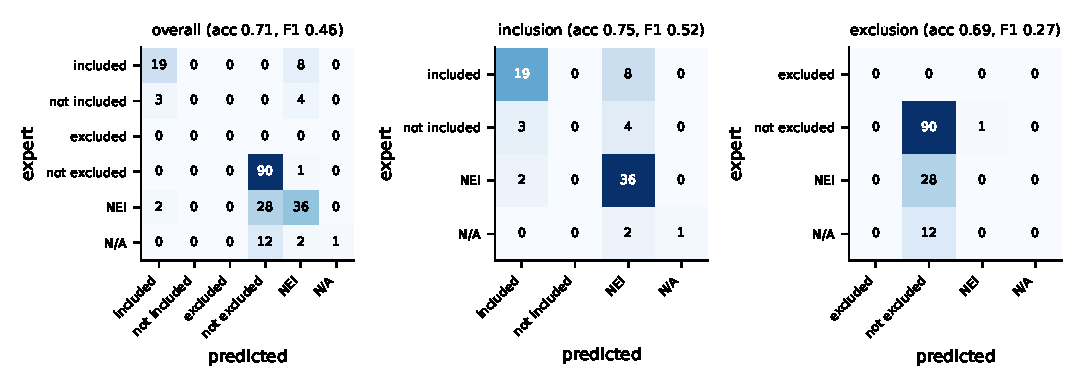
\includegraphics[width=.85\textwidth]{gpu_fig_confusion.pdf}
\caption{Config.~A confusion matrices on the test split (NEI = not enough information, N/A = not applicable).}\label{fig:cmA}\end{figure*}

\subsection{Evidence-Sentence Localisation (Config.~A)}
Table~\ref{tab:evA} reports sentence-ID precision, recall and F1. \NGoldEmpty{} of the \NTest{} test records have \emph{no} annotated evidence sentence and only \NGoldNon{} have at least one, which dominates every aggregate. With micro pooling the fine-tuned model reaches P~0.538, R~0.298, F1~\GTestEvF{} (interval \GTestEvFLo--\GTestEvFHi) against the base model's 0.151: the base model cites many sentences (recall 0.447, precision 0.091), the adapted model cites few but more correct ones. On evidence-bearing records the macro F1 is 0.277; if empty-gold records count as correct when nothing is cited, macro F1 rises to 0.757 purely because the model leaves 95.9\% of the empty-gold records empty (10 spurious citations in total), which shows why that second number must not be read as localisation skill. The split by type is telling: inclusion micro-F1 is 0.491 while exclusion micro-F1 is 0.000, because the model never cites a sentence for an exclusion criterion. Cited IDs are always valid sentence IDs of the note, and the application only displays text that exists in the note.

\begin{table}[t]\centering\caption{Config.~A evidence-sentence metrics on the test split (micro, and macro over evidence-bearing or all records).}\label{tab:evA}
\footnotesize\setlength{\tabcolsep}{3pt}\resizebox{\columnwidth}{!}{\begin{tabular}{llrrrr}\toprule
Model & Scope & P & R & F1 & Type \\\midrule
base & overall & 0.091 & 0.447 & 0.151 & micro \\
base & inclusion & 0.158 & 0.500 & 0.240 & micro \\
base & exclusion & 0.041 & 0.344 & 0.074 & micro \\
base & overall & 0.267 & 0.412 & 0.295 & macro (gold$\neq\emptyset$) \\
base & overall & 0.079 & 0.122 & 0.087 & macro (all records) \\\midrule
fine-tuned & overall & 0.538 & 0.298 & 0.384 & micro \\
fine-tuned & inclusion & 0.538 & 0.452 & 0.491 & micro \\
fine-tuned & exclusion & 0.000 & 0.000 & 0.000 & micro \\
fine-tuned & overall & 0.290 & 0.295 & 0.277 & macro (gold$\neq\emptyset$) \\
fine-tuned & overall & 0.761 & 0.762 & 0.757 & macro (all records) \\\bottomrule\end{tabular}
}\end{table}

\subsection{Error Analysis (Config.~A)}
\label{sec:errors}
Of the \NTest{} test criteria, \GNLabelErr{} (29\%) receive a wrong label and a further 35 have a correct label with a different evidence set; 111 are correct in both respects. Table~\ref{tab:errcatA} categorises every non-correct case and Table~\ref{tab:errA} lists twelve representative, distinct cases from different patients, trials and categories (full text in \texttt{results/error\_analysis\_gpu\_finetuned\_test.md}).

\emph{Missing information treated as ``not excluded''.} The largest category is false decision: 42 rows whose expert label is \emph{not enough information} (30) or \emph{not applicable} (12) but where the model commits to a decisive label; 40 of the 42 are exclusion criteria answered \emph{not excluded}. E1 (``Pregnancy'', expert: not applicable) and E3 (``BMI $>$ 40'', expert: not enough information) are typical: the note contains nothing about the topic and the model, instead of reporting the gap, defaults to the label that is correct most often. This is exactly the behaviour the task warns against---absence of evidence being read as eligibility---so \emph{not excluded} outputs without cited evidence should be shown to users as unverified, which the application does by displaying ``no supporting sentence cited''.

\emph{Uncited decisive predictions.} 130 test predictions carry a decisive label with no cited sentence. For 114 of them the expert also cites nothing, which is consistent with the dataset (about three quarters of \emph{not excluded} labels have empty evidence), but 16 have expert evidence that the model failed to cite (E4, E8): these are the contradictory cases where a label is given without the supporting sentence that exists in the note.

\emph{Missed decisions.} 13 rows have a decisive expert label but the model answers \emph{not enough information} (E7, E8): for example ``Shock or ARDS'' is marked \emph{included} by the expert based on hypotension and tachycardia (sentences 2--3), while the model says the note lacks information. These failures need clinical inference from vital signs, which a small model trained on 602 rows does not acquire.

\emph{Polarity flips and \emph{not applicable} confusions} are rare (3 and 2), and the \emph{not included} class (7 rows) is mostly answered \emph{included} (3) or \emph{not enough information} (4). \emph{Evidence-only} errors (35) divide into over-citation, where a \emph{not enough information} answer cites the first five sentences although the expert cites none (E5), and under-citation, where the single relevant sentence is missed (E6).

\begin{table}[t]\centering\caption{Config.~A test errors by category (all 206 rows; ``correct'' means label and evidence both match).}\label{tab:errcatA}
\small\begin{tabular}{lr}\toprule
Error category & Count \\\midrule
correct & 111 \\
false decision & 42 \\
evidence only & 35 \\
missed decision & 13 \\
polarity flip & 3 \\
na confusion & 2 \\
\bottomrule\end{tabular}
\end{table}
\begin{table*}[t]\centering\caption{Config.~A: twelve representative errors (evidence lists are sentence IDs; Expert/Model columns show label and IDs).}\label{tab:errA}
\scriptsize\begin{tabular}{p{.05\linewidth}p{.15\linewidth}p{.32\linewidth}p{.13\linewidth}p{.13\linewidth}}\toprule
ID & Type & Criterion (abridged) & Expert & Model \\\midrule
E1 & false decision & Pregnancy & not applicable [] & not excluded [] \\
E2 & false decision & Patients were moribund. & not enough info. [0, 1, 2, 3, 4] & not excluded [] \\
E3 & false decision & BMI> 40 kg/m2. & not enough info. [] & not excluded [] \\
E4 & evidence only & Had been performed central venous puncture or catheterization before. & not excluded [0] & not excluded [] \\
E5 & evidence only & bilateral pulmonary infiltrates or a chest radiograph consistent with edema; & not enough info. [] & not enough info. [0, 1, 2, 3, 4] \\
E6 & evidence only & Patients with liver space occupying lesion (LOE) that require extended hepatic resection. & not enough info. [3] & not enough info. [] \\
E7 & missed decision & Patients undergoing elective carotid endarterectomy & not included [] & not enough info. [] \\
E8 & missed decision & Patients were included if they were diagnosed with Shock, Acute respiratory distress syndr… & included [2, 3] & not enough info. [] \\
E9 & missed decision & Present with active SLE disease with at least one of the following symptoms: i) Arthritis … & included [0, 1] & not enough info. [] \\
E10 & polarity flip & Patients undergoing open abdominal aortic aneurysm repair & not included [] & included [0] \\
E11 & na confusion & If female, using birth control & not applicable [3] & not enough info. [] \\
E12 & na confusion & female patients have adequate birth-control method & not applicable [] & not enough info. [] \\
\bottomrule\end{tabular}
\end{table*}

\subsection{KV-Cached Generation (Config.~A)}
\label{sec:kvres}
Table~\ref{tab:kvA} compares the uncached reference, the explicit KV cache with PyTorch SDPA attention, and the cache combined with our tiled kernel for prompts of 64, 256 and 512 tokens and 16, 64 and 128 generated tokens on the T4, in fp32 on the 1.7B model. \textbf{Correctness:} the greedy token sequences of all three paths are identical in \GKVAllMatch{} configurations, including 512+128 tokens, even though the cached path multiplies a single query against the cache while the reference recomputes full matrices; no mismatch needed investigation, and the unit tests on smaller models additionally match the Hugging Face logits to $6\times10^{-5}$. \textbf{Speed:} prefill time is the same for all paths (0.09--0.7\,s, growing with prompt length) as expected, because prefill computes the same thing. Decode is where the cache matters: the uncached path re-reads and recomputes the whole prefix at every step, so its throughput (prefill included) is only 4.3--6.6 tokens/s for 64-token prompts and falls to 1.2--1.3 tokens/s for 512-token prompts, whereas the cached path stays between 14 and 30 tokens/s, i.e.\ \GKVSpeedup$\times$ faster end to end at 512+128 tokens (Fig.~\ref{fig:kvtimeA}). The cached tokens/s itself declines mildly with prompt length (30.1 at 64 tokens to 24.8 at 512) because every step attends to more cached keys. \textbf{Memory:} the cache is the price paid for this speed. The 1.7B model uses multi-head attention with 32 KV heads, so one cached token costs $2\cdot24\cdot32\cdot64\cdot4=393$\,kB in fp32 (the measured 239.6\,MB for 639 tokens agrees), and the measured peak allocation growth is 289--331\,MB with the cache versus 91--110\,MB without at 512 tokens (Fig.~\ref{fig:kvmemA}); this includes the pre-allocated buffer of 256 or more slots. For comparison, the grouped-query 360M model needs only 82\,kB per token. \textbf{Tiled attention inside the decoder:} the cached path with our tiled kernel produces identical tokens but is 1.6--4.5$\times$ slower than SDPA (5.5 vs.\ 24.8 tokens/s at 512+128) because every decode step runs a Python loop over key blocks, an overhead discussed next.

\begin{table*}[t]\centering\caption{Config.~A KV-cache benchmark (median of 3 repetitions after warm-up; peak $\Delta$ is the CUDA allocator peak above the pre-call level, KV = cache bytes in use; the last column checks token equality with the uncached reference).}\label{tab:kvA}
\small\begin{tabular}{rrlrrrrrc}\toprule
In & Out & Mode & Prefill (s) & Decode (s) & tok/s & Peak $\Delta$ (MB) & KV (MB) & = ref. \\\midrule
64 & 16 & uncached & 0.102 & 2.325 & 6.6 & 14 & 0.0 & yes \\
 &  & kv\_cache & 0.100 & 0.491 & 26.8 & 107 & 29.6 & yes \\
 &  & kv\_cache\_tiled & 0.094 & 0.884 & 16.4 & 107 & 29.6 & yes \\
64 & 64 & uncached & 0.125 & 12.331 & 5.1 & 22 & 0.0 & yes \\
 &  & kv\_cache & 0.089 & 2.024 & 30.2 & 107 & 47.6 & yes \\
 &  & kv\_cache\_tiled & 0.090 & 3.611 & 17.3 & 107 & 47.6 & yes \\
64 & 128 & uncached & 0.112 & 29.406 & 4.3 & 33 & 0.0 & yes \\
 &  & kv\_cache & 0.102 & 4.153 & 30.1 & 107 & 71.6 & yes \\
 &  & kv\_cache\_tiled & 0.105 & 8.277 & 15.3 & 107 & 71.6 & yes \\
256 & 16 & uncached & 0.327 & 6.490 & 2.3 & 47 & 0.0 & yes \\
 &  & kv\_cache & 0.334 & 0.511 & 18.9 & 149 & 101.6 & yes \\
 &  & kv\_cache\_tiled & 0.335 & 1.617 & 8.2 & 149 & 101.6 & yes \\
256 & 64 & uncached & 0.353 & 28.947 & 2.2 & 55 & 0.0 & yes \\
 &  & kv\_cache & 0.328 & 2.115 & 26.2 & 167 & 119.6 & yes \\
 &  & kv\_cache\_tiled & 0.351 & 6.659 & 9.1 & 167 & 119.6 & yes \\
256 & 128 & uncached & 0.347 & 60.917 & 2.1 & 66 & 0.0 & yes \\
 &  & kv\_cache & 0.328 & 4.308 & 27.6 & 191 & 143.6 & yes \\
 &  & kv\_cache\_tiled & 0.353 & 14.498 & 8.6 & 191 & 143.6 & yes \\
512 & 16 & uncached & 0.683 & 12.507 & 1.2 & 91 & 0.0 & yes \\
 &  & kv\_cache & 0.589 & 0.528 & 14.3 & 289 & 197.6 & yes \\
 &  & kv\_cache\_tiled & 0.669 & 2.623 & 4.9 & 289 & 197.6 & yes \\
512 & 64 & uncached & 0.656 & 49.965 & 1.3 & 99 & 0.0 & yes \\
 &  & kv\_cache & 0.612 & 2.217 & 22.6 & 307 & 215.6 & yes \\
 &  & kv\_cache\_tiled & 0.697 & 11.065 & 5.5 & 307 & 215.6 & yes \\
512 & 128 & uncached & 0.645 & 95.949 & 1.3 & 110 & 0.0 & yes \\
 &  & kv\_cache & 0.616 & 4.543 & 24.8 & 331 & 239.6 & yes \\
 &  & kv\_cache\_tiled & 0.714 & 22.456 & 5.5 & 331 & 239.6 & yes \\
\bottomrule\end{tabular}
\end{table*}
\begin{figure}[t]\centering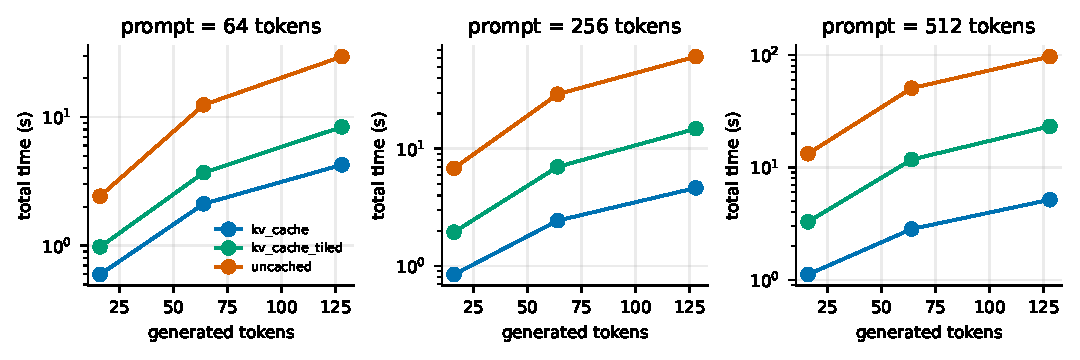
\includegraphics[width=\columnwidth]{gpu_fig_kv_time.pdf}
\caption{Config.~A: total generation time (log scale) against generated tokens for three prompt lengths.}\label{fig:kvtimeA}\end{figure}
\begin{figure}[t]\centering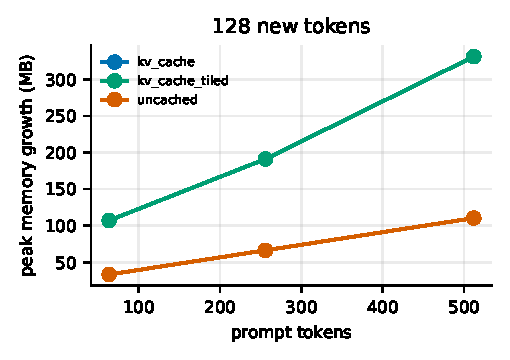
\includegraphics[width=.75\columnwidth]{gpu_fig_kv_memory.pdf}
\caption{Config.~A: peak allocation growth against prompt length at 128 new tokens.}\label{fig:kvmemA}\end{figure}

\subsection{Tiled Online-Softmax Attention (Config.~A)}
Table~\ref{tab:attnA} and Fig.~\ref{fig:attnA} validate and benchmark the kernels at the head shape of the 360M model (15 query heads, 5 KV heads, $d=64$) with random inputs. \textbf{Numerical agreement:} against the float32 reference the tiled kernel's maximum absolute error never exceeds $9.6\times10^{-7}$ across $T=128\ldots4096$ in prefill and $T=128\ldots2048$ in decode (worst error over all measured points, including SDPA: \GAttnWorstErr), with a mean error around $2\times10^{-8}$; unit tests add a hand-computed example, grouped heads, non-zero cache offsets, left padding and extreme score magnitudes where naive softmax overflows. \textbf{Memory:} the reference path's peak allocation grows quadratically (196\,MB at $T{=}1024$, 754\,MB at 2048, 2\,956\,MB at 4096) whereas the tiled kernel's grows roughly linearly (11, 22, 45\,MB), which is the intended effect of never forming the $T\times T$ score matrix. \textbf{Speed:} the tiled kernel is \emph{slower}: at $T{=}1024$ it needs 98\,ms against 5.9\,ms for the reference and 2.8\,ms for the fused SDPA kernel, and 1.6\,s against 83\,ms at 4096. This is expected for an educational PyTorch implementation: each tile launches half a dozen small kernels and Python-level loop iterations, reads and writes the running statistics from global memory, and cannot overlap data movement with compute as a fused FlashAttention-style kernel does with on-chip SRAM~\cite{dao2022flashattention}. The tile-size sweep supports this explanation (Fig.~\ref{fig:tileA}): at $T{=}1024$ the time drops from 1\,560\,ms with 16$\times$16 tiles to 98\,ms at 64, 30\,ms at 128 and 7.6\,ms at 256, nearly matching the reference, while the error is unchanged ($\le 9.5\times10^{-7}$)---the number of Python-level iterations, not arithmetic, dominates. In decode mode ($T_q{=}1$) there is no score matrix to save, so the reference (0.65\,ms) is even faster than SDPA (1.04\,ms) at $T{=}2048$, since both are launch-bound.

\begin{table}[t]\centering\caption{Config.~A attention benchmark: prefill ($T_q{=}T_k{=}T$) and decode ($T_q{=}1$) for three lengths; tiled uses 64$\times$64 tiles; errors are versus the reference.}\label{tab:attnA}
\footnotesize\setlength{\tabcolsep}{2.5pt}\resizebox{\columnwidth}{!}{\begin{tabular}{llrrrrr}\toprule
Phase & Impl. & $T$ & Time (ms) & Max err. & Mean err. & Peak $\Delta$ (MB) \\\midrule
prefill & reference & 256 & 1.01 & 0.0e+00 & 0.0e+00 & 15 \\
prefill & sdpa & 256 & 0.47 & 6.6e-07 & 3.1e-08 & 4 \\
prefill & tiled & 256 & 7.58 & 6.0e-07 & 2.7e-08 & 4 \\
prefill & reference & 1024 & 5.86 & 0.0e+00 & 0.0e+00 & 196 \\
prefill & sdpa & 1024 & 2.77 & 7.2e-07 & 3.0e-08 & 20 \\
prefill & tiled & 1024 & 98.06 & 8.3e-07 & 2.3e-08 & 11 \\
prefill & reference & 2048 & 20.25 & 0.0e+00 & 0.0e+00 & 754 \\
prefill & sdpa & 2048 & 12.13 & 6.9e-07 & 2.9e-08 & 50 \\
prefill & tiled & 2048 & 401.02 & 4.8e-07 & 2.2e-08 & 22 \\
\midrule
decode & reference & 256 & 0.67 & 0.0e+00 & 0.0e+00 & 2 \\
decode & sdpa & 256 & 0.36 & 1.5e-07 & 2.9e-08 & 2 \\
decode & tiled & 256 & 3.09 & 7.5e-08 & 1.1e-08 & 1 \\
decode & reference & 1024 & 0.66 & 0.0e+00 & 0.0e+00 & 8 \\
decode & sdpa & 1024 & 0.82 & 1.6e-07 & 2.6e-08 & 8 \\
decode & tiled & 1024 & 12.01 & 6.0e-08 & 9.5e-09 & 1 \\
decode & reference & 2048 & 0.65 & 0.0e+00 & 0.0e+00 & 15 \\
decode & sdpa & 2048 & 1.04 & 1.7e-07 & 2.4e-08 & 15 \\
decode & tiled & 2048 & 25.14 & 6.0e-08 & 9.2e-09 & 1 \\
\bottomrule\end{tabular}
}\end{table}
\begin{figure*}[t]\centering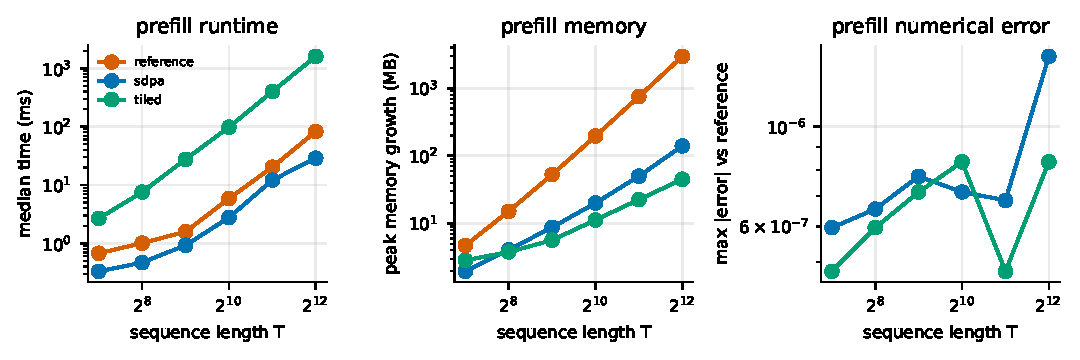
\includegraphics[width=.9\textwidth]{gpu_fig_attention.pdf}
\caption{Config.~A prefill attention: runtime, memory and error versus sequence length (log scales).}\label{fig:attnA}\end{figure*}
\begin{figure}[t]\centering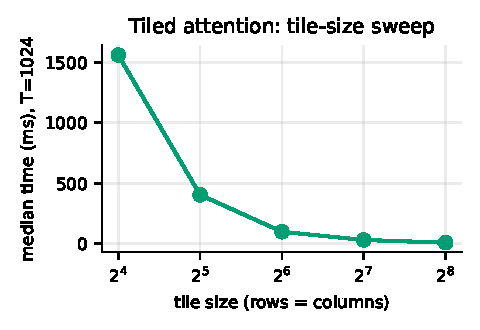
\includegraphics[width=.7\columnwidth]{gpu_fig_tile_sweep.pdf}
\caption{Config.~A: effect of tile size on tiled-attention time at $T=1024$.}\label{fig:tileA}\end{figure}

\subsection{Speculative Decoding (Config.~A)}
\label{sec:specres}
Tables~\ref{tab:specA1} and~\ref{tab:specA2} and Fig.~\ref{fig:specA} (acceptance and speed-up against the draft length $k$) compare cached greedy decoding of the 1.7B target against our speculative decoder with the fine-tuned 360M draft and with the un-tuned 360M draft, on 32 test prompts (speed only; no model selection used these prompts). \textbf{Correctness:} outputs are token-identical to greedy target decoding for \emph{every} prompt and every setting (32/32 in all 16 rows), and an independent check with Hugging Face assisted generation on six prompts agrees: \GSpecHF. \textbf{Acceptance:} with natural task output (about 13 tokens of JSON) the fine-tuned draft is accepted 92--98\% of the time, against 40--64\% for the un-tuned draft, so adapting the draft on the same task raises acceptance by 30--50 points; with forced 64-token outputs, where the continuation after the JSON is unconstrained, acceptance drops to 33--65\% for both drafts and the benefit of adaptation disappears. Acceptance falls with the draft length $k$ in all cases. \textbf{Latency:} despite high acceptance, speculative decoding is \emph{slower} than plain greedy decoding in every configuration: the best speed-up is \GSpecBestSpeedup$\times$ ($k{=}\GSpecBestK$, \GSpecBestDraft) for natural output and as low as 0.39$\times$ for forced long output. The cause is the cost ratio. On a GPU single-token decoding is limited by per-layer kernel launches and memory latency, not by arithmetic, so latency is roughly proportional to depth; the 360M draft has \emph{32} layers while the 1.7B target has only \emph{24}, so a draft step costs about as much as a target step. The speed-up model of Leviathan et al.~\cite{leviathan2023speculative}, $(1-\alpha^{k+1})/((1-\alpha)(kc+1))$, with draft/target cost ratio $c\approx1$, is below one for any acceptance rate. Our measured mean accepted length per round (5.8 tokens for the fine-tuned draft at $k{=}8$ on natural output, 2.3--2.5 for the un-tuned draft and for forced output) confirms that verification works as designed---the target needs well under one forward pass per emitted token (0.31 for forced output at $k{=}8$)---while draft cost cancels the gain. A faster configuration would need a much shallower draft (fewer layers) or a larger target. Memory is not an issue (extra allocation growth about 240\,MB, similar to the plain cache).

\begin{table}[t]\centering\caption{Config.~A speculative decoding, natural task output (32 prompts; Equal = outputs identical to greedy target; Accept. = accepted / proposed draft tokens).}\label{tab:specA1}
\footnotesize\begin{tabular}{llrrrrr}\toprule
Draft & $k$ & Equal & Accept. & Latency (s) & tok/s & Speed-up \\\midrule
\multicolumn{2}{l}{greedy target} & -- & -- & 0.894 & 15.0 & 1.00 \\\midrule
finetuned draft & 2 & 32/32 & 97\% & 1.180 & 11.4 & 0.76 \\
finetuned draft & 4 & 32/32 & 98\% & 1.133 & 11.8 & 0.79 \\
finetuned draft & 6 & 32/32 & 96\% & 1.102 & 12.2 & 0.81 \\
finetuned draft & 8 & 32/32 & 92\% & 1.110 & 12.1 & 0.81 \\
untuned draft & 2 & 32/32 & 64\% & 1.340 & 10.0 & 0.67 \\
untuned draft & 4 & 32/32 & 58\% & 1.370 & 9.8 & 0.65 \\
untuned draft & 6 & 32/32 & 49\% & 1.480 & 9.1 & 0.60 \\
untuned draft & 8 & 32/32 & 40\% & 1.630 & 8.2 & 0.55 \\
\bottomrule\end{tabular}
\end{table}
\begin{table}[t]\centering\caption{Config.~A speculative decoding, forced 64-token output.}\label{tab:specA2}
\footnotesize\begin{tabular}{llrrrrr}\toprule
Draft & $k$ & Equal & Accept. & Latency (s) & tok/s & Speed-up \\\midrule
\multicolumn{2}{l}{greedy target} & -- & -- & 2.571 & 24.9 & 1.00 \\\midrule
finetuned draft & 2 & 32/32 & 65\% & 4.230 & 15.1 & 0.61 \\
finetuned draft & 4 & 32/32 & 49\% & 4.798 & 13.3 & 0.54 \\
finetuned draft & 6 & 32/32 & 39\% & 5.743 & 11.1 & 0.45 \\
finetuned draft & 8 & 32/32 & 33\% & 6.547 & 9.8 & 0.39 \\
untuned draft & 2 & 32/32 & 63\% & 4.304 & 14.9 & 0.60 \\
untuned draft & 4 & 32/32 & 52\% & 4.629 & 13.8 & 0.56 \\
untuned draft & 6 & 32/32 & 41\% & 5.543 & 11.5 & 0.46 \\
untuned draft & 8 & 32/32 & 33\% & 6.471 & 9.9 & 0.40 \\
\bottomrule\end{tabular}
\end{table}
\begin{figure*}[t]\centering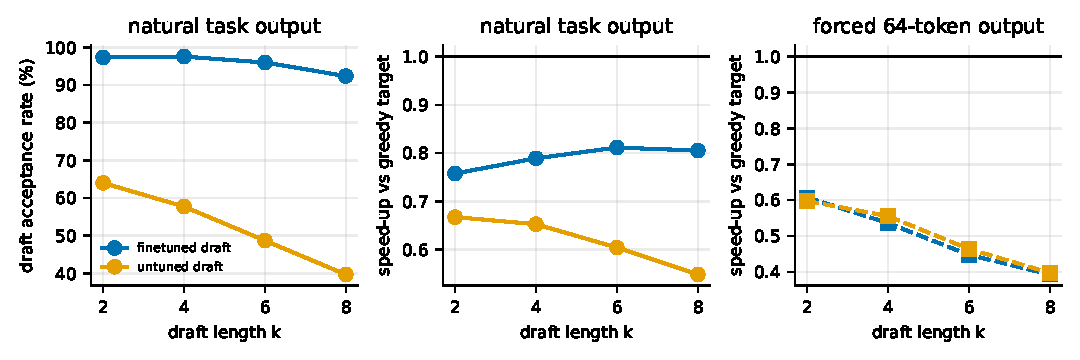
\includegraphics[width=.9\textwidth]{gpu_fig_speculative.pdf}
\caption{Config.~A: acceptance rate and speed-up against draft length $k$ for the fine-tuned and un-tuned draft.}\label{fig:specA}\end{figure*}

\subsection{Configuration B: CPU Laptop Model}
\label{sec:cpu}
Configuration~B repeats the experiment on the laptop CPU with SmolLM2-360M as target (8.68M LoRA parameters, 2 epochs, \TTrainHours{}\,h of training) and SmolLM2-135M as draft. It matters for two reasons: it is the model the locally hosted application loads by default, and it shows how much of Configuration~A's behaviour depends on model scale.

\textbf{Fine-tuning and before/after.} Table~\ref{tab:epochsB} and Fig.~\ref{fig:trainB} show that after epoch~1 the model's validation accuracy (0.621) and macro-F1 (0.215) are \emph{identical} to the majority-label baseline: it had learned the answer format and the common label, nothing more. After epoch~2 (selected, validation macro-F1 0.317) it has started to discriminate inclusion classes. Table~\ref{tab:mainB} gives the before/after comparison on identical rows. The zero-shot 360M base model reaches test accuracy \BaseAcc{} and macro-F1 \BaseMF{} (it follows the schema, 0 invalid outputs, but cites no evidence at all: evidence F1 0.000); after fine-tuning, accuracy is \TestAcc{} (interval \TestAccLo--\TestAccHi), macro-F1 \TestMF{} (interval \TestMFLo--\TestMFHi) and micro evidence F1 \TestEvF{} (interval \TestEvFLo--\TestEvFHi). \textbf{This is the same accuracy as the majority baseline} (\MajAcc{}), and the macro-F1 interval contains the baseline's \MajMF{}; with 8 test patients we therefore cannot claim a reliable improvement over trivial prediction for this configuration, only a point-estimate gain in macro-F1 (0.333 vs.\ 0.272) driven by inclusion criteria. Validation shows the same picture (0.684 accuracy and 0.317 macro-F1 against 0.621 and 0.215 for the majority label).

\textbf{Per-class behaviour.} For exclusion criteria the fine-tuned model answers \emph{not excluded} on all 131 rows, i.e.\ it reproduces the majority label exactly (exclusion accuracy 0.695, macro-F1 0.273), and for inclusion criteria it answers \emph{not enough information} 57 times and \emph{included} 18 times (Table~\ref{tab:pcBcpu}, Fig.~\ref{fig:cmB}): \emph{included} reaches only P~0.44, R~0.30, F1~0.36 against 0.79, 0.70 and 0.75 for the 1.7B model, and \emph{not included} and \emph{not applicable} are never predicted. \emph{Not enough information} for inclusion criteria is its best class (F1 0.63).

\textbf{Evidence.} Micro precision is 0.350 but recall only 0.074 (inclusion: P~0.350, R~0.113, F1~0.171; exclusion: nothing cited); on evidence-bearing records the macro F1 is 0.109, whereas the all-record macro F1 of 0.707 merely reflects that the model leaves \EmptyOK{} of the empty-gold records empty (\EmptyFalseCit{} spurious citations).

\textbf{Errors.} Of \NTest{} test rows 101 are correct in label and evidence, 50 are false decisions (gold \emph{not enough information} 36 or \emph{not applicable} 14, answered \emph{not excluded} 40 times and \emph{included} 10 times), 28 have the right label with different evidence, 26 are missed decisions (a decisive gold label answered \emph{not enough information} or \emph{not applicable}) and 1 is a \emph{not applicable} confusion (Table~\ref{tab:errcatB}); 131 predictions carry a decisive label without any cited sentence, 115 of which also have empty expert evidence and 16 of which do not. The twelve-case listing for Configuration~A (Table~\ref{tab:errA}) illustrates the same failure types; the CPU cases are in \texttt{results/error\_analysis\_cpu\_finetuned\_test.md}. The comparison with Configuration~A suggests that, on this data, a 1.7B model with three epochs begins to learn inclusion reasoning (included recall 0.70 vs.\ 0.30, evidence micro-F1 0.384 vs.\ 0.123) whereas a 360M model with two epochs mostly learns the label prior; both collapse on exclusion criteria.

\begin{table}[t]\centering\caption{Config.~B target (SmolLM2-360M + LoRA, CPU): validation after each epoch ($^*$ = selected).}\label{tab:epochsB}
\small\begin{tabular}{rrrrr}\toprule
Epoch & Val. loss & Val. acc. & Val. macro-F1 & Val. evid. F1 \\\midrule
1 & 0.207 & 0.621 & 0.215 & 0.214 \\
2$^*$ & 0.189 & 0.684 & 0.317 & 0.196 \\
\bottomrule\end{tabular}
\end{table}
\begin{figure}[t]\centering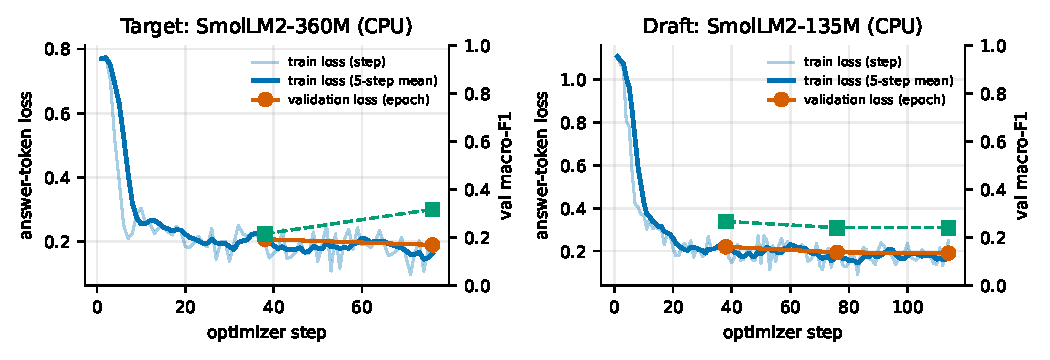
\includegraphics[width=\columnwidth]{fig_training.pdf}
\caption{Config.~B training curves (CPU): target 360M and draft 135M.}\label{fig:trainB}\end{figure}
\begin{table*}[t]\centering\caption{Config.~B (CPU): majority baseline, base zero-shot and fine-tuned SmolLM2-360M on the same rows.}\label{tab:mainB}
\small\begin{tabular}{llrrrrrrr}\toprule
Split & Model & Acc. & mF1 & Incl. acc. & Incl. mF1 & Excl. acc. & Excl. mF1 & Invalid \\\midrule
Val. & majority label & 0.621 & 0.215 & 0.409 & 0.145 & 0.721 & 0.210 & 0 \\
& base zero-shot & 0.495 & 0.229 & 0.136 & 0.113 & 0.664 & 0.276 & 0 \\
& fine-tuned & 0.684 & 0.317 & 0.606 & 0.310 & 0.721 & 0.210 & 0 \\
\midrule
Test & majority label & 0.626 & 0.272 & 0.507 & 0.168 & 0.695 & 0.273 & 0 \\
& base zero-shot & 0.437 & 0.234 & 0.120 & 0.070 & 0.618 & 0.350 & 0 \\
& fine-tuned & 0.626 & 0.333 & 0.507 & 0.247 & 0.695 & 0.273 & 0 \\
\bottomrule\end{tabular}
\end{table*}
\begin{table}[t]\centering\caption{Config.~B fine-tuned model, test split: per-class P, R, F1 and support.}\label{tab:pcBcpu}
\footnotesize\begin{tabular}{llrrrr}\toprule
Scope & Class & P & R & F1 & Support \\\midrule
inclusion & included & 0.444 & 0.296 & 0.356 & 27 \\
 & not included & 0.000 & 0.000 & 0.000 & 7 \\
 & not enough info. & 0.526 & 0.789 & 0.632 & 38 \\
 & not applicable & 0.000 & 0.000 & 0.000 & 3 \\
\midrule
exclusion & excluded & 0.000 & 0.000 & 0.000 & 0 \\
 & not excluded & 0.695 & 1.000 & 0.820 & 91 \\
 & not enough info. & 0.000 & 0.000 & 0.000 & 28 \\
 & not applicable & 0.000 & 0.000 & 0.000 & 12 \\
\bottomrule\end{tabular}
\end{table}
\begin{figure*}[t]\centering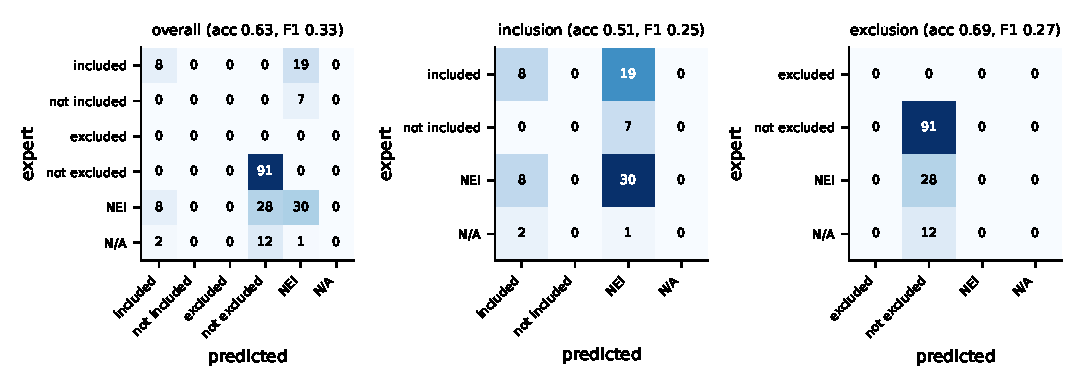
\includegraphics[width=.85\textwidth]{fig_confusion.pdf}
\caption{Config.~B confusion matrices on the test split.}\label{fig:cmB}\end{figure*}
\begin{table}[t]\centering\caption{Config.~B test errors by category.}\label{tab:errcatB}
\small\begin{tabular}{lr}\toprule
Error category & Count \\\midrule
correct & 101 \\
false decision & 50 \\
evidence only & 28 \\
missed decision & 26 \\
na confusion & 1 \\
\bottomrule\end{tabular}
\end{table}

\textbf{Draft model (SmolLM2-135M).} Table~\ref{tab:epochsBd} shows the draft's validation behaviour over three epochs (\DTrainHours{}\,h on the CPU). Validation loss keeps falling (0.220, 0.194, 0.191), but the selection rule (highest validation macro-F1) picks epoch~\DBestEpoch{} (0.267) because macro-F1 is higher there than at epochs 2 and 3 (both 0.241); the differences are a few points on 206 rows and are not meaningful beyond showing that the 135M model learns the answer format and the label prior and little else. This is acceptable for a draft, whose purpose is to propose the target's likely tokens, not to be accurate by itself, but it means that the acceptance rates of the CPU pair were not benchmarked in a stored table (see below) and should not be inferred from the GPU pair.

\textbf{What the laptop is used for.} Configuration~B provides the model of the locally hosted application, whose \emph{Compare decoding} tab measures all four decoding modes live on the user's CPU (Section~\ref{sec:appres}); we did not run the full stored benchmark grid of Section~\ref{sec:kvres}--\ref{sec:specres} on the CPU, because the GPU grid already covers prompt lengths, output lengths, attention shapes and draft settings with a larger, more realistic model and any CPU table would add timings but no new correctness evidence. CPU-specific numbers should therefore be taken from the live tab rather than from this paper.

\begin{table}[t]\centering\caption{Config.~B draft (SmolLM2-135M + LoRA, CPU): validation after each epoch ($^*$ = selected).}\label{tab:epochsBd}
\small\begin{tabular}{rrrrr}\toprule
Epoch & Val. loss & Val. acc. & Val. macro-F1 & Val. evid. F1 \\\midrule
1$^*$ & 0.220 & 0.636 & 0.267 & 0.175 \\
2 & 0.194 & 0.631 & 0.241 & 0.048 \\
3 & 0.191 & 0.631 & 0.241 & 0.254 \\
\bottomrule\end{tabular}
\end{table}



\subsection{Application}
\label{sec:appres}
The application is a self-contained web service: \texttt{python app/server.py} (or \texttt{run\_app.bat}) starts a FastAPI server on \texttt{127.0.0.1:8000}, loads the target and draft models and merges the LoRA adapters in a background thread, and serves a single-page browser interface; no notebook, command-line step or IDE is needed afterwards. The header shows a status indicator (starting, ready, error), the loaded model and adapter, and a persistent banner states that this is an educational screening prototype and not a clinical enrollment decision. Loading takes well under a minute on the laptop; requests that arrive earlier receive a clear ``model not ready'' message instead of an error. If an adapter is missing, the base model is used and the header says so.

\textbf{Screening workflow (Fig.~\ref{fig:app2}).} A user supplies a patient note by pasting text or loading one of the held-out sample patients, and a trial by choosing a sample trial, fetching one from ClinicalTrials.gov by NCT identifier (public metadata only), pasting an ``Inclusion Criteria / Exclusion Criteria'' block that is split into individual criteria, or typing criteria manually. Notes that are not already numbered are split into sentences and numbered from zero, with a preview of the numbering. For every criterion the interface shows the predicted label, the cited sentences quoted from the note, an explanation that only restates the label and the cited text, the raw model output, latency and generated tokens, and, for the sample patients, the dataset's expert label with a match indicator; selecting a criterion highlights its cited sentences in the numbered note (yellow) and the expert's sentences (green marker). The preliminary outcome (here ``Needs more information'') is computed by the explicit rule of Section~III-H and is displayed together with that rule. Missing information is never presented as eligibility: a criterion with no cited sentence is shown with the text ``No supporting sentence cited''.

\textbf{Report export and provenance.} The \emph{Download report} buttons produce a readable HTML report (also suitable for printing to PDF), a Markdown file or a JSON file containing the disclaimer, the trial, the preliminary outcome with its rule, every criterion with label, evidence text and explanation, the numbered note, and provenance: generation time, model, a SHA-256 prefix of the adapter file, the decoding settings and a hash of the note.

\textbf{Input validation and recovery (Fig.~\ref{fig:app3}).} The server validates every request: notes shorter than 20 characters, unknown criterion types, criteria shorter than 3 characters or empty reports are rejected with an explanatory message and HTTP~422; an unreachable registry yields a message asking the user to paste the criteria instead; prompts above 3\,000 tokens are refused rather than silently truncated; and if one criterion fails during a multi-criterion run it is reported as invalid while the others continue. After an error the user corrects the field and runs again without reloading.

\textbf{Inference comparison (Fig.~\ref{fig:app4}).} The \emph{Compare decoding} tab runs the current note and a chosen criterion through the four implemented modes---uncached reference, KV cache, KV cache with tiled attention, and speculative decoding with a selectable draft length---with a warm-up pass and selectable repetitions, optionally forcing a longer output. It reports whether each mode's tokens are identical to the first, prefill, decode and total time, tokens per second, speed-up, memory growth, target forward passes and, for speculative decoding, the acceptance rate, and draws latency and throughput bars. These numbers are measured live on the machine hosting the application, not read from images; the \emph{Experiments} tab additionally renders the stored result files (before/after metrics, KV, attention and speculative benchmarks). In the screenshot, taken while a training job was competing for the same CPU, all four modes return identical tokens, the cache is faster than the reference, our tiled kernel is slower than SDPA inside the decoder, and speculative decoding reaches a 41\% acceptance rate with the un-tuned draft available at that moment.

\begin{figure}[t]\centering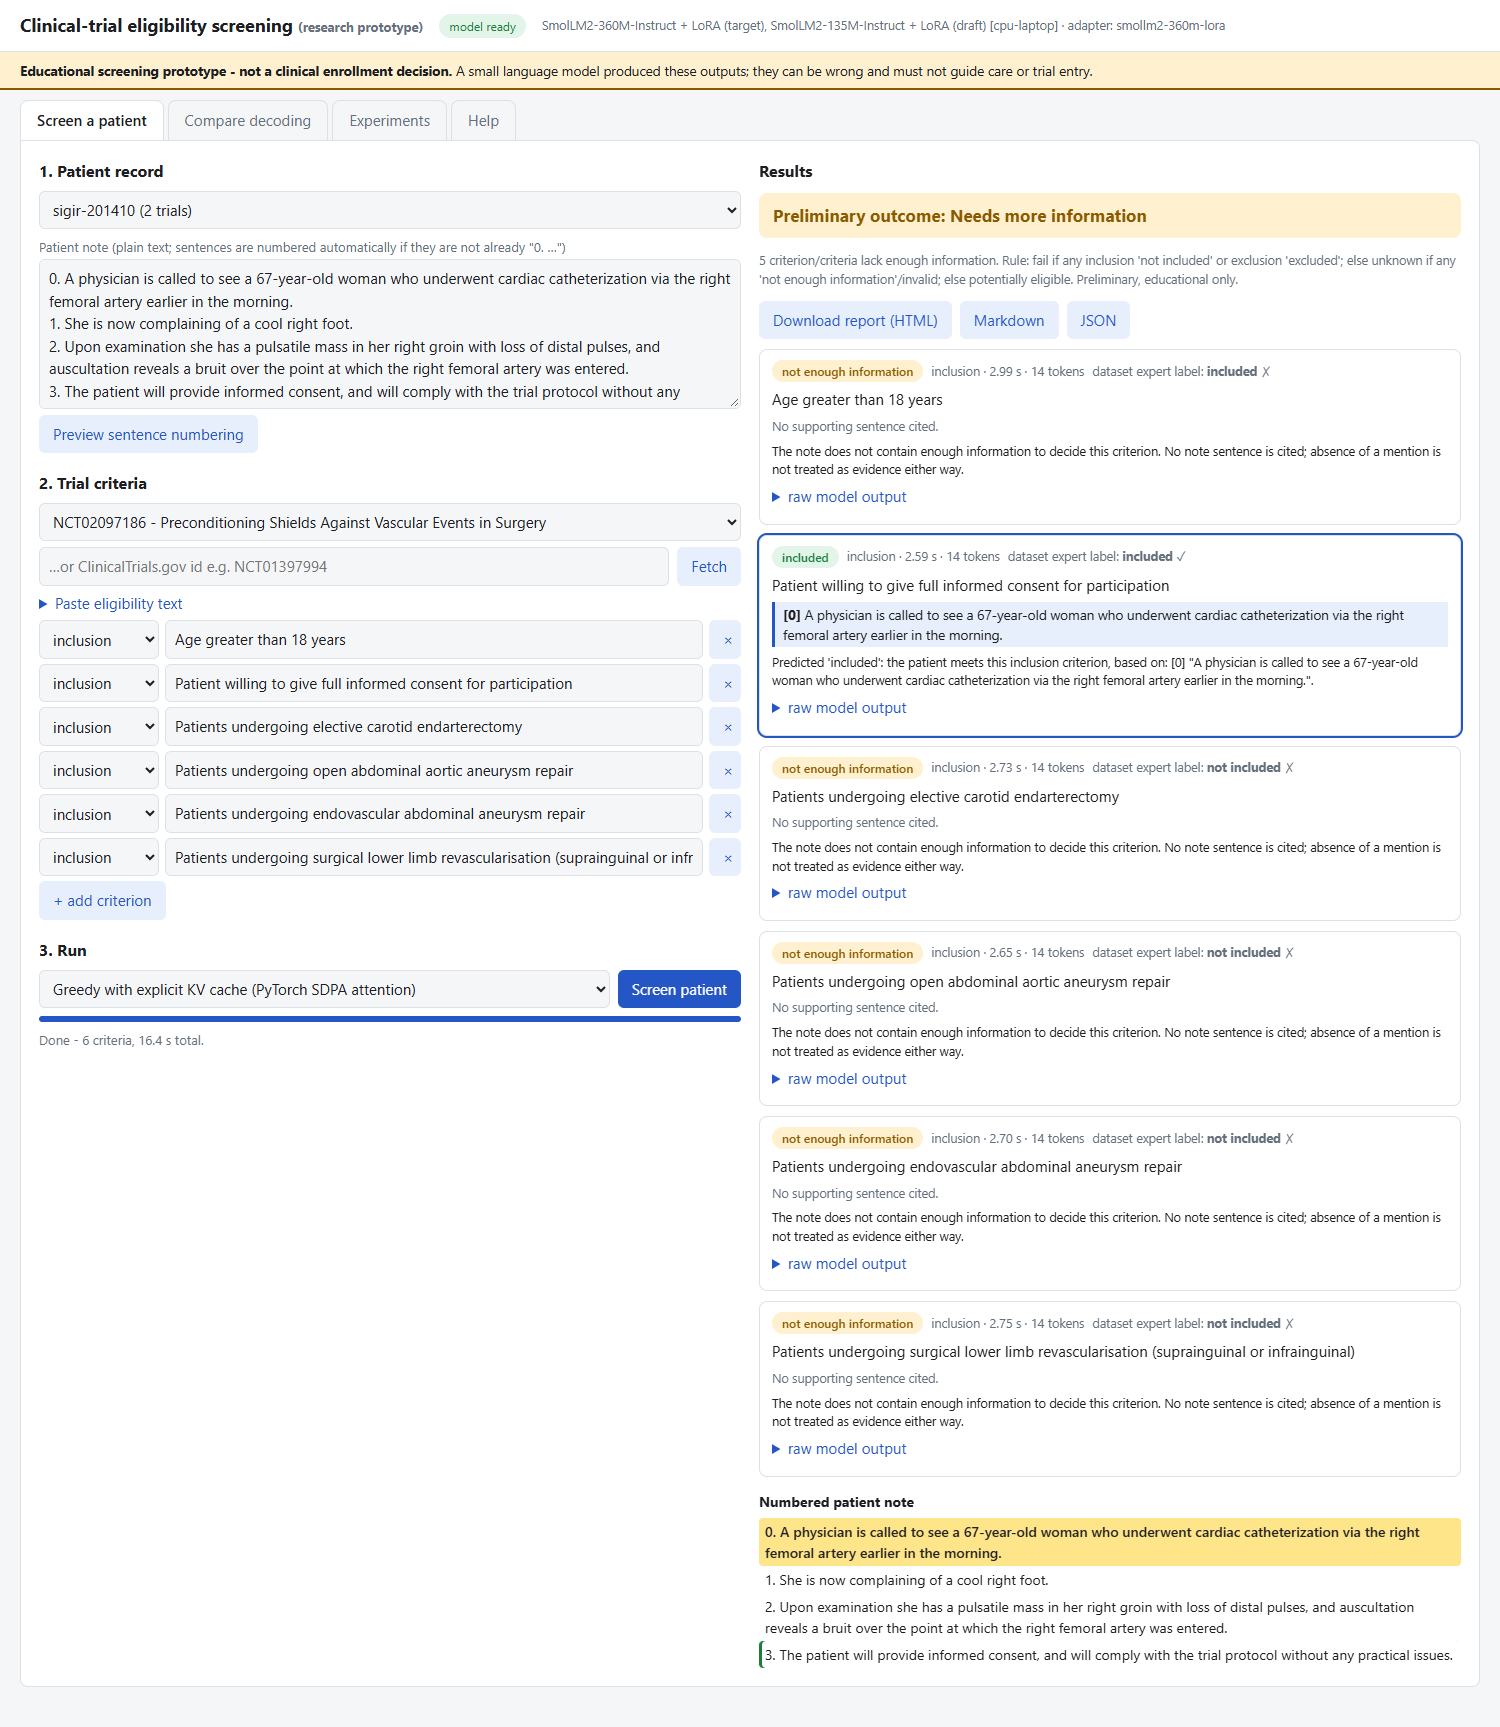
\includegraphics[height=.52\textheight,keepaspectratio]{app_02_results.png}
\caption{Screening workflow: sample patient and trial, six criteria screened, per-criterion label and cited evidence, preliminary outcome, report export buttons, and the numbered note with the selected criterion's evidence highlighted.}\label{fig:app2}\end{figure}
\begin{figure}[t]\centering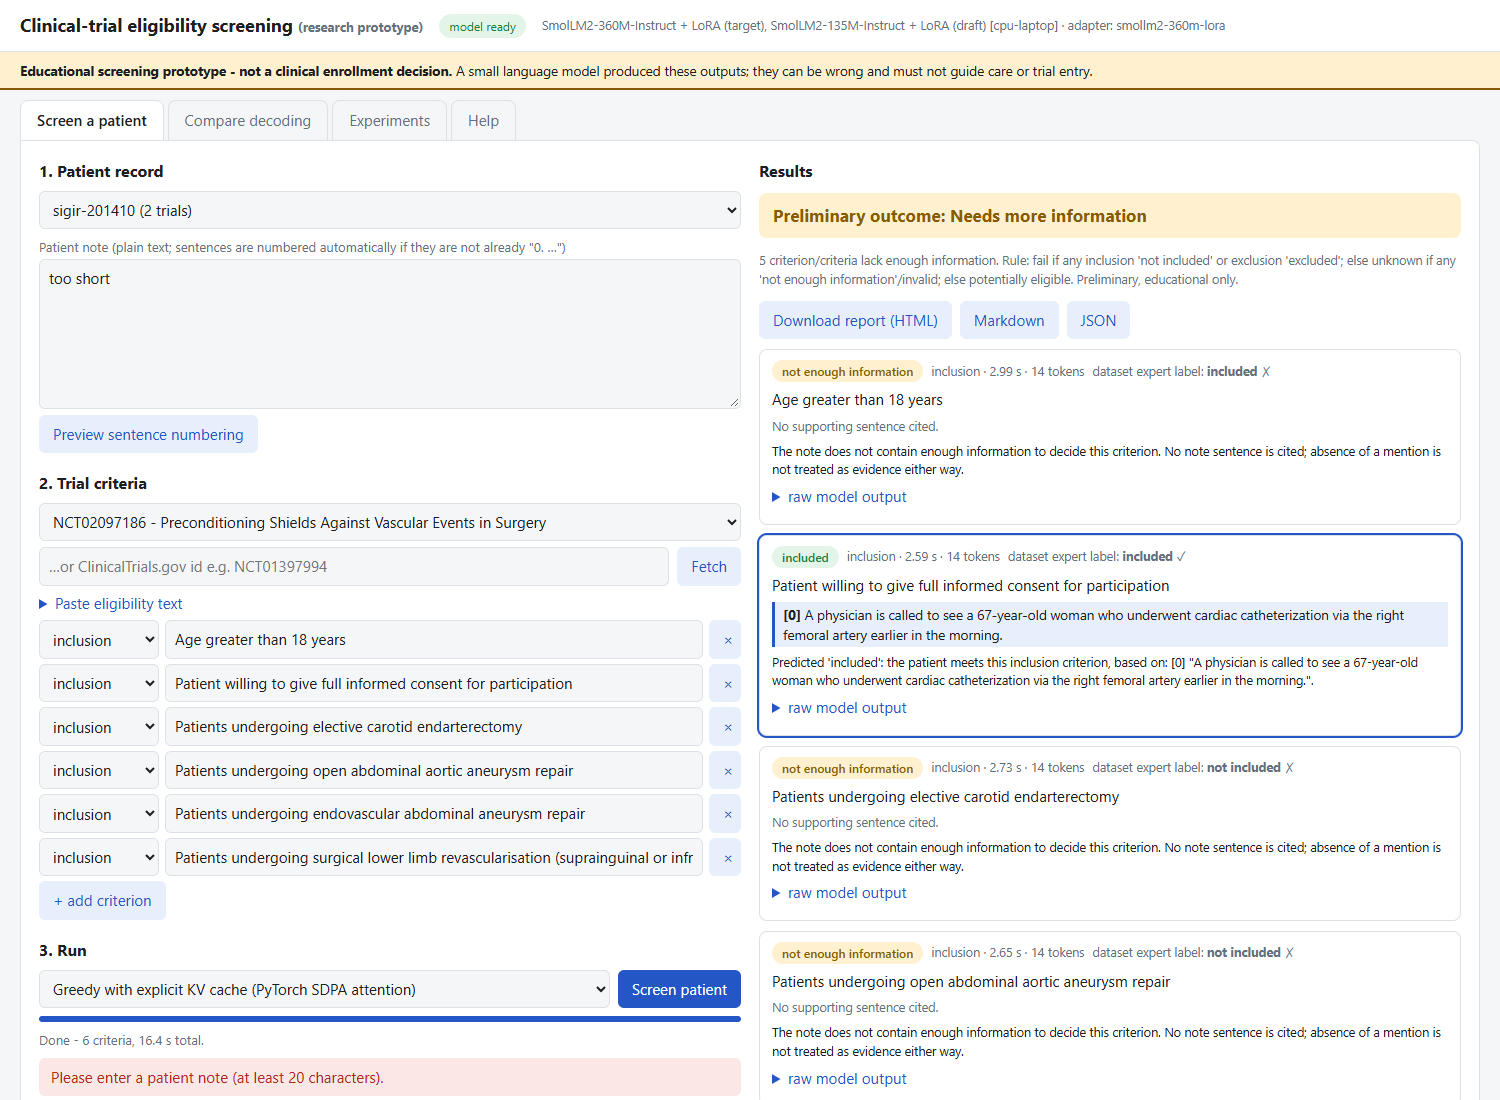
\includegraphics[width=\columnwidth]{app_03_error_recovery.png}
\caption{Recovery from an invalid input: a too-short note is rejected with an explanatory message and the form remains usable.}\label{fig:app3}\end{figure}
\begin{figure}[t]\centering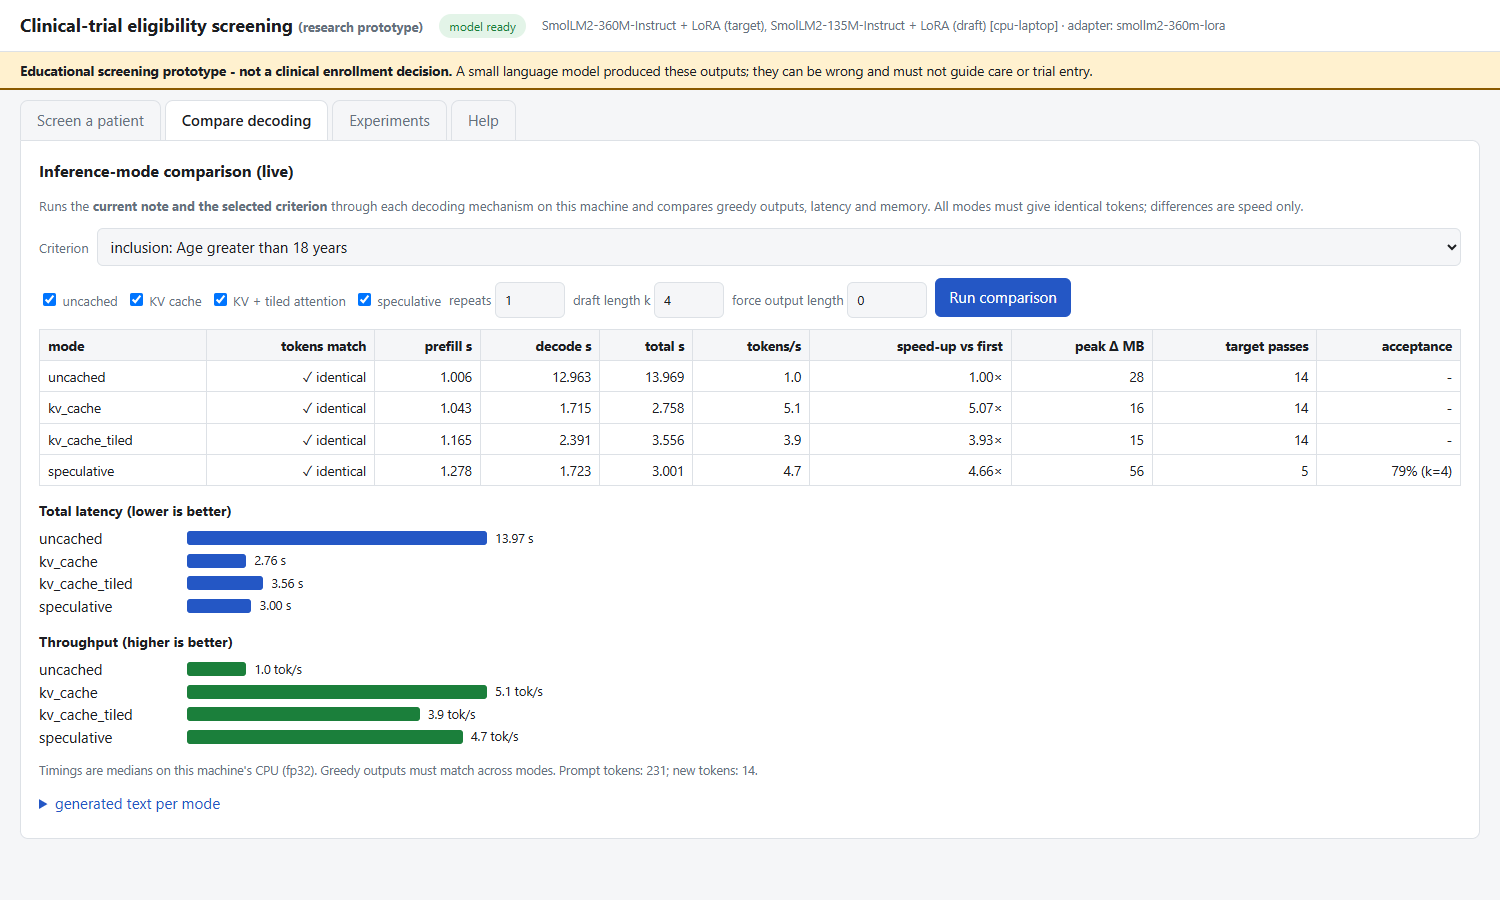
\includegraphics[width=\columnwidth]{app_04_compare.png}
\caption{\emph{Compare decoding} tab: live comparison of the four decoding modes on the same input (timings include contention from a concurrent training job).}\label{fig:app4}\end{figure}

